\newpage
\section{Marco teórico}
\subsection{Ferromagnetismo}

%El proceso de magnetización espontanea depende de las propiedades intrinsecas e extrinsecas del material.

El ferromagnetismo es un fenómeno físico, de tipo magnético, presente en ciertos materiales. Consiste en un comportamiento ordenado, en ciertas regiones (dominios magnéticos) del material, de sus momentos magnéticos (Figura \ref{fig:MagneticDomain}). Este comportamiento se caracteriza por su magnetización espontánea, $\bm{M}$. Dicha magnetización depende fuertemente de la estructura cristalina del sólido, ya que los momentos dipolares magnéticos tienden a alinearse en los ejes  ``fáciles'' \cite{coey_2010}. En el micromagnetismo clásico, la magnitud de la magnetización, para una temperatura fija $T$, es constante, es decir, queda totalmente caracterizada por sus cosenos directores \cite{Exl2020} \[ \bm{M} (\bm{r},T) = \mu_0 \bm{J}_s = |M (T)| (\gamma_1 (\bm{r}) \hat{e}_1 + \gamma_2 (\bm{r}) \hat{e}_2 + \gamma_3 (\bm{r}) \hat{e}_3 ), \] en donde $\gamma_i$ son los cosenos directores referidos a algún sistema de referencia ortogonal con vectores unitarios $\hat{e}_k$; $\bm{J}_s$ es la polarización espontánea y $\mu_0$ la permeabilidad magnética del vacío.
\begin{figure}[!htp]
    \centering
    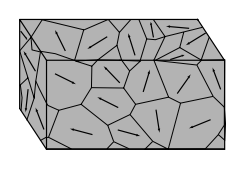
\includegraphics{Figuras/MagneticDomain.png}
    \renewcommand{\figurename}{\textbf{Figura}}
    \renewcommand\thefigure{\textbf{\arabic{figure}}}
    \caption{Dominios magnéticos en un sólido ferromagnético \cite{coey_2010}.}
    \label{fig:MagneticDomain}
\end{figure}
\subsection{Términos de energía magnéticos}
En el micromagnetismo, la relación básica para el estudio del fenómeno magnético es la densidad de energía libre de Gibbs, $\phi'_l$, la cual se puede escribir como \[ \phi'_l = U - T S - \sigma \cdot \epsilon - \bm{J}_s \cdot \bm{H}_{ext},\] en donde $S$ es la densidad de entropía; $U$ la densidad de energía interna; $\epsilon$ el tensor de estrés. Además, $U$ contiene los términos de densidad de energía de intercambio, anisotropía magnetocristalina y magnetostática. Las variables libres son la temperatura $T$, el tensor elástico $\sigma$ y el campo externo aplicado $\bm{H}_{ext}$ \cite{KronmüllerMicromagnetism,Exl2020}. La energía libre de Gibbs total en equilibrio térmico está dada por \[ \phi_l = \int \phi'_l ~ dV .\]
\subsubsection{Energía de intercambio}
El Hamiltoniano de intercambio de Heisenberg modela las interacciones de intercambio de los electrones desapareados, usualmente de los átomos vecinos más próximos \cite{coey_2010}, el cual podemos escribir de forma general como \[ \mathcal{H}_{ex} = - 2 \sum_{i \neq j} J_{ij} \bm{S}_i \cdot \bm{S}_j ,\] en donde $J_{ij}$ es la integral de intercambio y $\bm{S}_k$ son los operadores de espín.

\vspace{10pt}

En el micromagnetismo, la derivación de una expresión continua para las interacciones de intercambio, entre los vecinos más próximos, parte del modelo de Heisenberg. En donde se considera a los operadores $\bm{S}_k$ como vectores clásicos y el ángulo entre ellos cambia muy lentamente y de forma continua\cite{Exl2020}. La densidad de energía de intercambio, $\phi'_{ex}$, se puede escribir como \[ \phi'_{ex} = A \sum_{n=1}^3 (\nabla \gamma_n (\bm{r}) )^2 ,\] en donde $A$ se le conoce como la constante de intercambio y depende en gran medida, entre otras cosas, de la estructura cristalina. 

%Incluir la constantes de intercambio para las simetrias cubicas y hcp.

\subsubsection{Energía magnetostática}
La energía magnetostática consta de dos términos: la energía Zeeman y la energía dipolar.

\vspace{10pt}

\textbf{Energía Zeeman}\\
La energía Zeeman o también llamada energía magnetostática del campo externo, surge de la interacción de los momentos magnéticos electrónicos con el campo externo aplicado \cite{Exl2020}. Se puede expresar la densidad de energía Zeeman como \[ \phi'_H = - \mu_0 \bm{H}_{ext} \cdot \bm{M}.\]

\textbf{Energía Dipolar}\\
En los sólidos cristalinos, cada momento dipolar produce un campo dipolar y cada uno de estos interaccionan con el campo producido por los demás dipolos magnéticos, $\bm{H}_s$. Como el campo magnético es generado sólo por los momentos dipolares se tiene $\nabla \times \bm{H}_s = 0$ y por tanto se le puede asociar un potencial escalar $\bm{H}_s = - \nabla U$ \cite{KronmüllerMicromagnetism}. La energía dipolar toma la forma \[ \phi_s = \frac{1}{2} \mu_0 \oint_{S_0} \sigma(\bm{r}) U(\bm{r}) d \bm{S} + \frac{1}{2} \mu_0 \int_{V_0} \rho (\bm{r}) U(\bm{r}) dV ,\] donde $\sigma(\bm{r}) = \bm{M} (\bm{r}) \cdot \hat{\bm{n}}$ es la densidad superficial de carga magnética; $\rho(\bm{r}) = - \nabla \cdot \bm{M} (\bm{r})$ la densidad volumétrica de carga magnética y $S_0$ la superficie que contiene al volumen $V_0$ del sistema. Equivalentemente, se puede expresar la densidad de energía dipolar como \[ \phi'_s = \frac{\mu_0}{2} \bm{H}_s^2 .\]

\subsubsection{Energía de anisotropía magnetocristalina}
%La anisotropía magnetocristalina es un caso particular de anisotropia magnética donde las propiedades magneticas se ven afectadas por la estructura cristalina.

%La energia de anisotroía magnetocristalina está asociada con el hecho de que, en general, en los materiales magneticos existen direcciónes para los cuales son más fácilmente magnetizables que en otras, esto es, que el campo magnético necesario para magnetizar el material hasta la saturación es menor en unas direcciones que en otras. En la dirección en donde el material es fácilemtne magnetizables decimos que es un "eje fácil" y en la dirección de dificil magnetización decimos que es un "eje duro".

La energía de anisotropía magnetocristalina está asociada con el hecho de que la magnetización en un dominio magnético, generalmente, tiende a orientarse a lo largo de ejes ``fáciles'' (Figura \ref{fig:Anisotropy}) \cite{coey_2010}. Una expresión general para la densidad de energía, $\phi'_K$, puede escribirse como \cite{birss1964symmetry} \[ \phi'_K = k_0 (\bm{r}) + \sum_{i \neq j} k_{ij} \gamma_i (\bm{r}) \gamma_j(\bm{r}) + \sum_{ijk} k_{ijk} \gamma_i (\bm{r}) \gamma_j (\bm{r}) \gamma_k (\bm{r}) + \dotsc,  \] en donde los $k$ son tensores de propiedades del material.
\begin{figure}[!hpt]
    \centering
    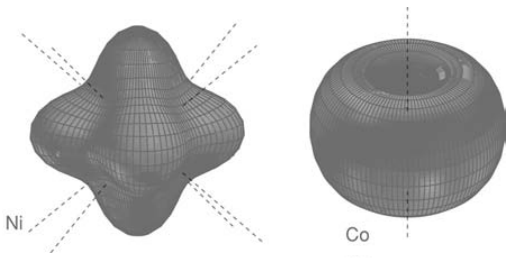
\includegraphics[scale=0.55]{Figuras/Anisotropy.png}
    \renewcommand{\figurename}{\textbf{Figura}}
    \renewcommand\thefigure{\textbf{\arabic{figure}}}
    \caption{Superficies de energía de anisotropía magnetocristalina para el cobalto y el níquel. El cobalto tiene un eje ``fácil'' y el níquel cuatro \cite{coey_2010}.}
    \label{fig:Anisotropy}
\end{figure}
\subsection{Ecuaciones de Landau-Lifshitz y Gilbert}
Las ecuaciones de Landau-Lifshitz y Gilbert (LLG) describen la evolución en el tiempo de la magnetización espontánea \cite{Exl2020} \[ \frac{d \bm{M}}{dt} = \gamma_G (\bm{M} \times \bm{H}_{eff}) - \frac{\alpha_G}{M}(\bm{M} \times \frac{d \bm{M}}{dt}),\] en donde $\gamma_G$ es la relación giromagnética de los electrones; $\alpha_G$ la constante de amortiguamiento de Gilbert y $\bm{H}_{eff} = - (1/J_s) \partial \phi_l / \partial \bm{m}$ con $\bm{m} = \bm{M}/M$. 
\subsection{Simulaciones micromagnéticas}
\subsubsection{Métodos numéricos}
Las ecuaciones LLG son un conjunto de ecuaciones no lineales acopladas por lo que obtener expresiones analíticas puede ser muy laborioso o incluso imposible. Así pues, se realizan aproximaciones numéricas para estudiar la dinámica de la magnetización. Los métodos más comunes son el micromagnetismo numérico de diferencias finitas (FE), basado en campo y el basado en energía, y el método de elemento finito (FD). El método FE basado en campo consiste en buscar la solución numérica sobre la base de una evaluación directa de las componentes del campo efectivo $\bm{H}_{eff}$ bajo la restricción de las condiciones de frontera. El método FE basado en energía se da prioridad a la energía magnética y se calcula directamente de la magnetización discretizada, mientras que el campo efectivo se deriva de la energía resultante \cite{miltat2007numerical}. El método FD consiste en que el dominio se subdivide en elementos y se aproximan las cantidades de campo usando funciones nodales \cite{FiniteElement}.

\subsubsection{Paquetes principales}
Existen una gran cantidad de paquetes de software de propósito general diseñados para resolver las ecuaciones LLG (Tabla \ref{tab:SoftwarePackage}). A grandes rasgos, las diferencias más importantes de estos paquetes son el método que usan para resolver las ecuaciones LLG, el hardware en el que corren (CPU o GPU) y si son de acceso gratuito o comercial\cite{Tomorrow}. En este trabajo de investigación nos centraremos en dos paquetes gratuitos muy populares: OOMMF y mumax$^3$.

\newpage
\begin{table}[htp!]
    \centering
    \begin{tabular}{|l|c|c|c|}
        \hline
        \textbf{Nombre} & \textbf{FE/FD} & \textbf{CPU/GPU} & \textbf{Gratis?} \\ \hline
        LLG & FD & CPU & No \\ \hline
        OOMF & FD & CPU & Si \\ \hline
        micromagus & FD & CPU & No \\ \hline
        magpar & FE & CPU & Si \\ \hline
        Nmag & FE & CPU & Si \\ \hline
        GPMagnet & FD & GPU & No \\ \hline
        FEMME & FE & CPU & No \\ \hline
        tetramaf$^b$ & FE & GPU & No \\ \hline 
        finmag$^c$ & FE & CPU & Si \\ \hline
        Fastmag & FE & GPU & No \\ \hline
        Mumax & FD & GPU & Si \\ \hline
        micromagnum & FD & GPU & Si \\ \hline
        magnum.fd$^d$ & FD & GPU & Si \\ \hline
        magnum.fe & FE & CPU & No \\ \hline
        mumax$^3$ & FD & GPU & Si \\ \hline
    \end{tabular}
    \renewcommand{\tablename}{\textbf{Tabla}}
    \renewcommand\thetable{\textbf{\arabic{table}}}
    \caption{Lista de paquetes de software de propósito general \cite{Tomorrow}.}
    \label{tab:SoftwarePackage}
\end{table}

\subsection{Ciclos de histéresis}
El fenómeno de histéresis consiste en la respuesta no lineal e irreversible de la magnetización con el campo aplicado, es decir, la magnetización espontánea no sigue una relación unívoca con el campo aplicado y depende, en gran medida, de las características intrínsecas e historia de preparación del material (Figura \ref{fig:hysteresis})\cite{coey_2010,jackson2012classical}. Además, en nanohilos magnéticos cilíndricos, este ciclo de histéresis también está influenciado por la orientación del campo magnético aplicado al mismo\cite{CylindricalMagneticNonowires}.

\begin{figure}[!htp]
    \centering
    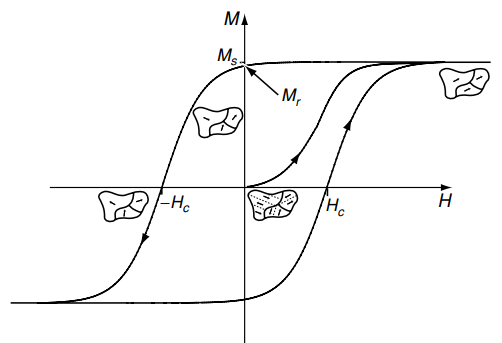
\includegraphics[scale=0.5]{Figuras/Hysteresis.png}
    \renewcommand{\figurename}{\textbf{Figura}}
    \renewcommand\thefigure{\textbf{\arabic{figure}}}
    \caption{Ciclo de histéresis de un ferromagnetico. En la imagen se ilustra el comportamiento de los dominos magnéticos cuando es magnetizado hasta la saturación $M_s$ y cuando es aplicado un campo $H_c$ (campo coersitivo) para la anulación de la imanación después de la saturación\cite{coey_2010}.}
    \label{fig:hysteresis}
\end{figure}

\subsection{Nanohilos ferromagnéticos de Co-Ni con anisotropía transversal}
Este sistema de nanohilos individuales se caracteriza por la aparición de una cadena de vórtices repartidos uniformemente a lo largo de la región $C2$ (Figura \ref{fig:ExoticVortexNW}). En dicha región, el flujo magnético rota alrededor de ejes fijos equidistantes. Además, la dirección de giro, horaria o antioraria, del flujo magnético cambia de forma alternada. En este sistema, conviven dos fases cristalográficas: hcp y fcc. En donde, se emplean una aleación de $\ce{Co}$-$\ce{Ni}$ con poca concentración de $\ce{Ni}$ para orientar eje fácil uniaxial, propio de la estructura hcp, perpendicular al eje del nanohilo. De esta forma, vencer la anisotropía de forma que tiende a orientar la magnetización a lo largo del eje del nanohilo \cite{ExoticMagneticConfiguration}.

\begin{figure}[!hpt]
    \centering
    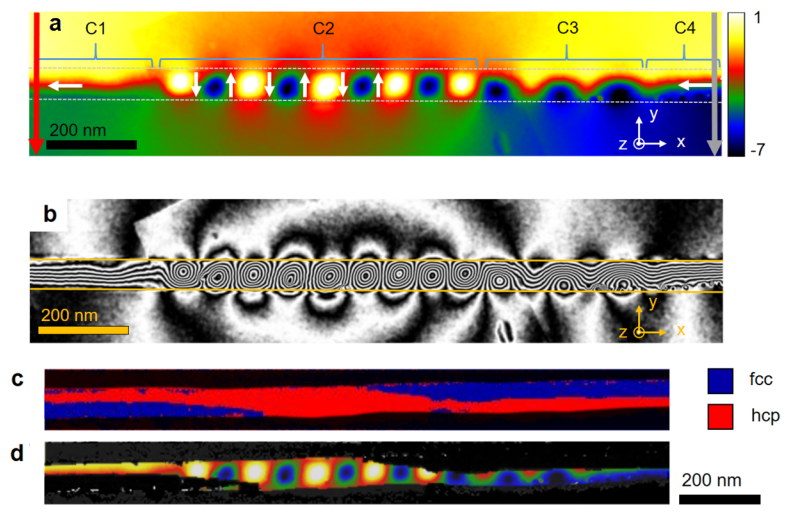
\includegraphics[scale=0.7]{Figuras/ExoticVortexNW.png}
    \caption{La figura a) muestra el cambio de fase magnética y b) muestra las lineas de flujo magnetico. Las gráficas c) y d) corresponden a resultados experimentales del analisis estructural del nanohilo. La Figura c) muestra las fases cristalográficas fcc y hpc en la dirección z al eje del nanohilo. La figura d) muestra la superposición de las figuras a) y c) en donde solo la fase hcp es visible \cite{ExoticMagneticConfiguration}}
    \label{fig:ExoticVortexNW}
\end{figure}